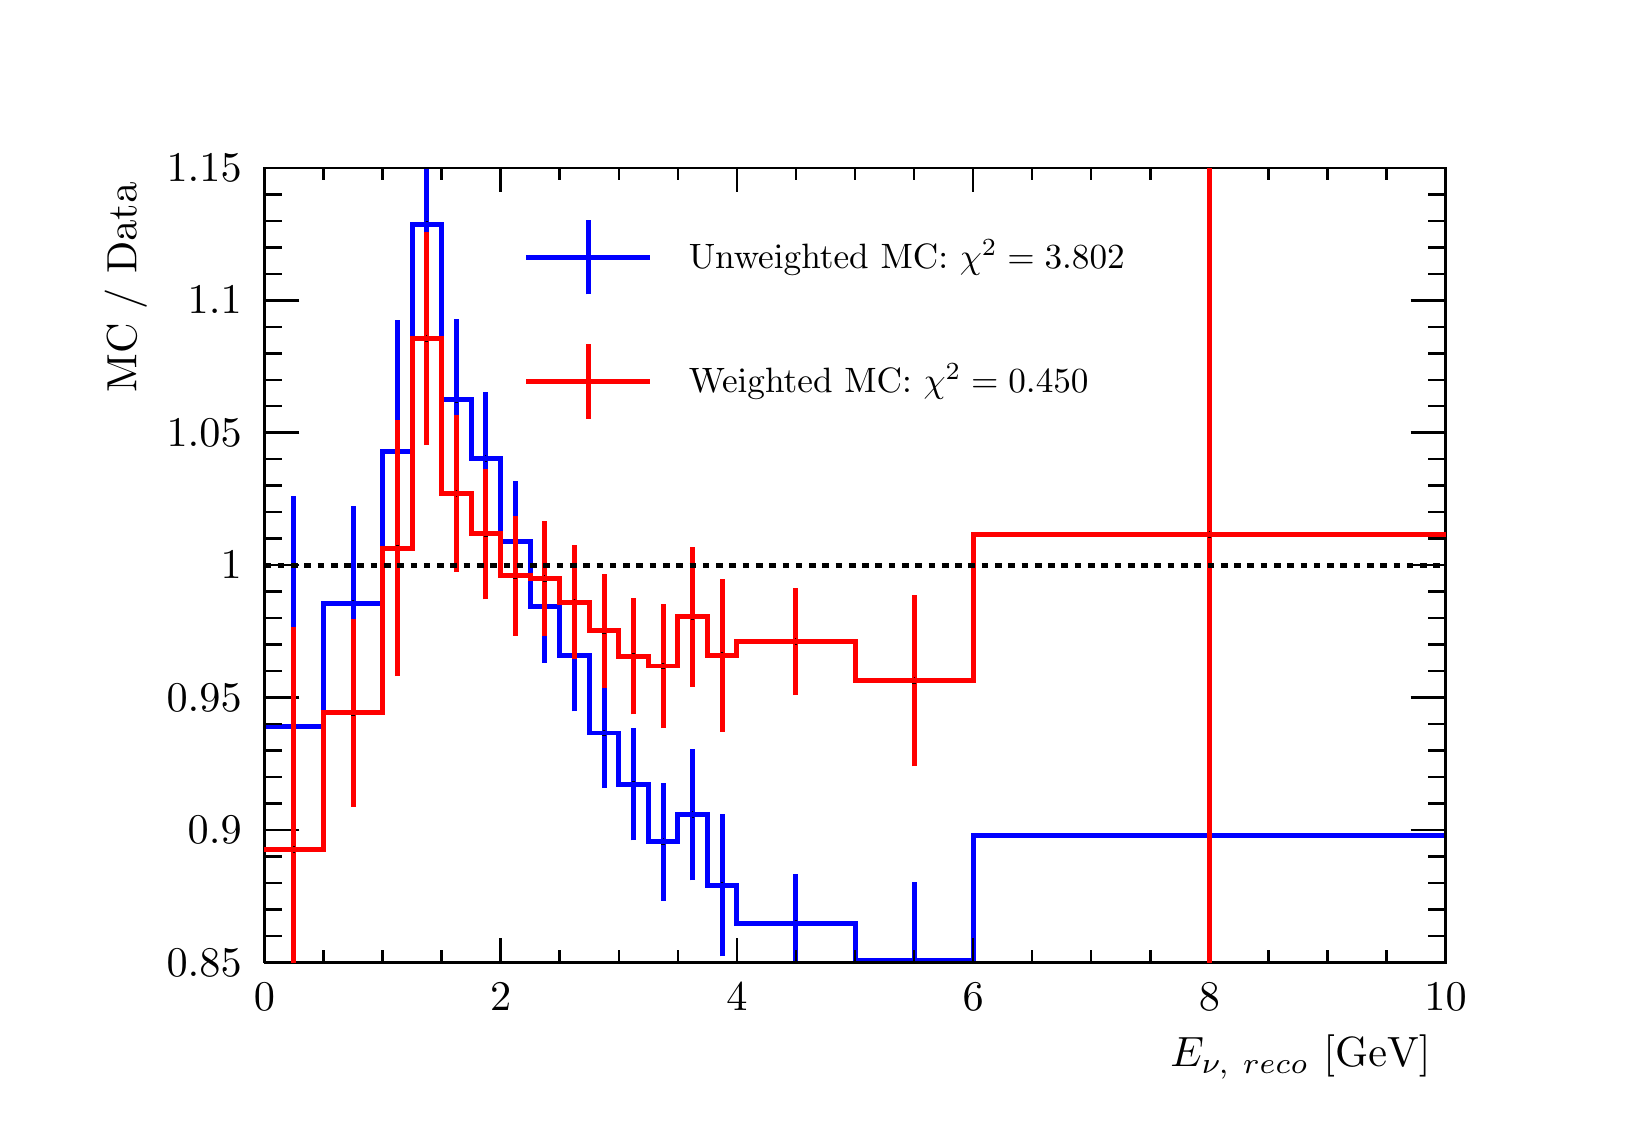
\begin{tikzpicture}
\pgfdeclareplotmark{cross} {
\pgfpathmoveto{\pgfpoint{-0.3\pgfplotmarksize}{\pgfplotmarksize}}
\pgfpathlineto{\pgfpoint{+0.3\pgfplotmarksize}{\pgfplotmarksize}}
\pgfpathlineto{\pgfpoint{+0.3\pgfplotmarksize}{0.3\pgfplotmarksize}}
\pgfpathlineto{\pgfpoint{+1\pgfplotmarksize}{0.3\pgfplotmarksize}}
\pgfpathlineto{\pgfpoint{+1\pgfplotmarksize}{-0.3\pgfplotmarksize}}
\pgfpathlineto{\pgfpoint{+0.3\pgfplotmarksize}{-0.3\pgfplotmarksize}}
\pgfpathlineto{\pgfpoint{+0.3\pgfplotmarksize}{-1.\pgfplotmarksize}}
\pgfpathlineto{\pgfpoint{-0.3\pgfplotmarksize}{-1.\pgfplotmarksize}}
\pgfpathlineto{\pgfpoint{-0.3\pgfplotmarksize}{-0.3\pgfplotmarksize}}
\pgfpathlineto{\pgfpoint{-1.\pgfplotmarksize}{-0.3\pgfplotmarksize}}
\pgfpathlineto{\pgfpoint{-1.\pgfplotmarksize}{0.3\pgfplotmarksize}}
\pgfpathlineto{\pgfpoint{-0.3\pgfplotmarksize}{0.3\pgfplotmarksize}}
\pgfpathclose
\pgfusepathqstroke
}
\pgfdeclareplotmark{cross*} {
\pgfpathmoveto{\pgfpoint{-0.3\pgfplotmarksize}{\pgfplotmarksize}}
\pgfpathlineto{\pgfpoint{+0.3\pgfplotmarksize}{\pgfplotmarksize}}
\pgfpathlineto{\pgfpoint{+0.3\pgfplotmarksize}{0.3\pgfplotmarksize}}
\pgfpathlineto{\pgfpoint{+1\pgfplotmarksize}{0.3\pgfplotmarksize}}
\pgfpathlineto{\pgfpoint{+1\pgfplotmarksize}{-0.3\pgfplotmarksize}}
\pgfpathlineto{\pgfpoint{+0.3\pgfplotmarksize}{-0.3\pgfplotmarksize}}
\pgfpathlineto{\pgfpoint{+0.3\pgfplotmarksize}{-1.\pgfplotmarksize}}
\pgfpathlineto{\pgfpoint{-0.3\pgfplotmarksize}{-1.\pgfplotmarksize}}
\pgfpathlineto{\pgfpoint{-0.3\pgfplotmarksize}{-0.3\pgfplotmarksize}}
\pgfpathlineto{\pgfpoint{-1.\pgfplotmarksize}{-0.3\pgfplotmarksize}}
\pgfpathlineto{\pgfpoint{-1.\pgfplotmarksize}{0.3\pgfplotmarksize}}
\pgfpathlineto{\pgfpoint{-0.3\pgfplotmarksize}{0.3\pgfplotmarksize}}
\pgfpathclose
\pgfusepathqfillstroke
}
\pgfdeclareplotmark{newstar} {
\pgfpathmoveto{\pgfqpoint{0pt}{\pgfplotmarksize}}
\pgfpathlineto{\pgfqpointpolar{44}{0.5\pgfplotmarksize}}
\pgfpathlineto{\pgfqpointpolar{18}{\pgfplotmarksize}}
\pgfpathlineto{\pgfqpointpolar{-20}{0.5\pgfplotmarksize}}
\pgfpathlineto{\pgfqpointpolar{-54}{\pgfplotmarksize}}
\pgfpathlineto{\pgfqpointpolar{-90}{0.5\pgfplotmarksize}}
\pgfpathlineto{\pgfqpointpolar{234}{\pgfplotmarksize}}
\pgfpathlineto{\pgfqpointpolar{198}{0.5\pgfplotmarksize}}
\pgfpathlineto{\pgfqpointpolar{162}{\pgfplotmarksize}}
\pgfpathlineto{\pgfqpointpolar{134}{0.5\pgfplotmarksize}}
\pgfpathclose
\pgfusepathqstroke
}
\pgfdeclareplotmark{newstar*} {
\pgfpathmoveto{\pgfqpoint{0pt}{\pgfplotmarksize}}
\pgfpathlineto{\pgfqpointpolar{44}{0.5\pgfplotmarksize}}
\pgfpathlineto{\pgfqpointpolar{18}{\pgfplotmarksize}}
\pgfpathlineto{\pgfqpointpolar{-20}{0.5\pgfplotmarksize}}
\pgfpathlineto{\pgfqpointpolar{-54}{\pgfplotmarksize}}
\pgfpathlineto{\pgfqpointpolar{-90}{0.5\pgfplotmarksize}}
\pgfpathlineto{\pgfqpointpolar{234}{\pgfplotmarksize}}
\pgfpathlineto{\pgfqpointpolar{198}{0.5\pgfplotmarksize}}
\pgfpathlineto{\pgfqpointpolar{162}{\pgfplotmarksize}}
\pgfpathlineto{\pgfqpointpolar{134}{0.5\pgfplotmarksize}}
\pgfpathclose
\pgfusepathqfillstroke
}
\definecolor{c}{rgb}{1,1,1};
\draw [color=c, fill=c] (0,0) rectangle (20,13.639);
\draw [color=c, fill=c] (3,1.77307) rectangle (18,11.8659);
\definecolor{c}{rgb}{0,0,0};
\draw [c,line width=0.9] (3,1.77307) -- (3,11.8659) -- (18,11.8659) -- (18,1.77307) -- (3,1.77307);
\definecolor{c}{rgb}{1,1,1};
\draw [color=c, fill=c] (3,1.77307) rectangle (18,11.8659);
\definecolor{c}{rgb}{0,0,0};
\draw [c,line width=0.9] (3,1.77307) -- (3,11.8659) -- (18,11.8659) -- (18,1.77307) -- (3,1.77307);
\definecolor{c}{rgb}{0,0,1};
\draw [c,line width=1.8] (3.375,1.8456) -- (3.375,4.77087);
\draw [c,line width=1.8] (3.375,4.77087) -- (3.375,7.69614);
\definecolor{c}{rgb}{0,0,0};
\foreach \P in {(3.375,4.77087)}{\draw[mark options={color=c,fill=c},mark size=2.402402pt, line width=0.000000pt, mark=*,mark size=1pt] plot coordinates {\P};}
\definecolor{c}{rgb}{0,0,1};
\draw [c,line width=1.8] (4.125,5.11119) -- (4.125,6.3386);
\draw [c,line width=1.8] (4.125,6.3386) -- (4.125,7.56602);
\definecolor{c}{rgb}{0,0,0};
\foreach \P in {(4.125,6.3386)}{\draw[mark options={color=c,fill=c},mark size=2.402402pt, line width=0.000000pt, mark=*,mark size=1pt] plot coordinates {\P};}
\definecolor{c}{rgb}{0,0,1};
\draw [c,line width=1.8] (4.6875,6.59132) -- (4.6875,8.2631);
\draw [c,line width=1.8] (4.6875,8.2631) -- (4.6875,9.93489);
\definecolor{c}{rgb}{0,0,0};
\foreach \P in {(4.6875,8.2631)}{\draw[mark options={color=c,fill=c},mark size=2.402402pt, line width=0.000000pt, mark=*,mark size=1pt] plot coordinates {\P};}
\definecolor{c}{rgb}{0,0,1};
\draw [c,line width=1.8] (5.0625,9.76007) -- (5.0625,11.1519);
\draw [c,line width=1.8] (5.0625,11.1519) -- (5.0625,11.8659);
\definecolor{c}{rgb}{0,0,0};
\foreach \P in {(5.0625,11.1519)}{\draw[mark options={color=c,fill=c},mark size=2.402402pt, line width=0.000000pt, mark=*,mark size=1pt] plot coordinates {\P};}
\definecolor{c}{rgb}{0,0,1};
\draw [c,line width=1.8] (5.4375,7.89664) -- (5.4375,8.91997);
\draw [c,line width=1.8] (5.4375,8.91997) -- (5.4375,9.9433);
\definecolor{c}{rgb}{0,0,0};
\foreach \P in {(5.4375,8.91997)}{\draw[mark options={color=c,fill=c},mark size=2.402402pt, line width=0.000000pt, mark=*,mark size=1pt] plot coordinates {\P};}
\definecolor{c}{rgb}{0,0,1};
\draw [c,line width=1.8] (5.8125,7.32529) -- (5.8125,8.17418);
\draw [c,line width=1.8] (5.8125,8.17418) -- (5.8125,9.02306);
\definecolor{c}{rgb}{0,0,0};
\foreach \P in {(5.8125,8.17418)}{\draw[mark options={color=c,fill=c},mark size=2.402402pt, line width=0.000000pt, mark=*,mark size=1pt] plot coordinates {\P};}
\definecolor{c}{rgb}{0,0,1};
\draw [c,line width=1.8] (6.1875,6.34375) -- (6.1875,7.11476);
\draw [c,line width=1.8] (6.1875,7.11476) -- (6.1875,7.88576);
\definecolor{c}{rgb}{0,0,0};
\foreach \P in {(6.1875,7.11476)}{\draw[mark options={color=c,fill=c},mark size=2.402402pt, line width=0.000000pt, mark=*,mark size=1pt] plot coordinates {\P};}
\definecolor{c}{rgb}{0,0,1};
\draw [c,line width=1.8] (6.5625,5.57956) -- (6.5625,6.30079);
\draw [c,line width=1.8] (6.5625,6.30079) -- (6.5625,7.02203);
\definecolor{c}{rgb}{0,0,0};
\foreach \P in {(6.5625,6.30079)}{\draw[mark options={color=c,fill=c},mark size=2.402402pt, line width=0.000000pt, mark=*,mark size=1pt] plot coordinates {\P};}
\definecolor{c}{rgb}{0,0,1};
\draw [c,line width=1.8] (6.9375,4.96311) -- (6.9375,5.67152);
\draw [c,line width=1.8] (6.9375,5.67152) -- (6.9375,6.37993);
\definecolor{c}{rgb}{0,0,0};
\foreach \P in {(6.9375,5.67152)}{\draw[mark options={color=c,fill=c},mark size=2.402402pt, line width=0.000000pt, mark=*,mark size=1pt] plot coordinates {\P};}
\definecolor{c}{rgb}{0,0,1};
\draw [c,line width=1.8] (7.3125,3.98807) -- (7.3125,4.68826);
\draw [c,line width=1.8] (7.3125,4.68826) -- (7.3125,5.38844);
\definecolor{c}{rgb}{0,0,0};
\foreach \P in {(7.3125,4.68826)}{\draw[mark options={color=c,fill=c},mark size=2.402402pt, line width=0.000000pt, mark=*,mark size=1pt] plot coordinates {\P};}
\definecolor{c}{rgb}{0,0,1};
\draw [c,line width=1.8] (7.6875,3.32593) -- (7.6875,4.03969);
\draw [c,line width=1.8] (7.6875,4.03969) -- (7.6875,4.75345);
\definecolor{c}{rgb}{0,0,0};
\foreach \P in {(7.6875,4.03969)}{\draw[mark options={color=c,fill=c},mark size=2.402402pt, line width=0.000000pt, mark=*,mark size=1pt] plot coordinates {\P};}
\definecolor{c}{rgb}{0,0,1};
\draw [c,line width=1.8] (8.0625,2.55826) -- (8.0625,3.30708);
\draw [c,line width=1.8] (8.0625,3.30708) -- (8.0625,4.05591);
\definecolor{c}{rgb}{0,0,0};
\foreach \P in {(8.0625,3.30708)}{\draw[mark options={color=c,fill=c},mark size=2.402402pt, line width=0.000000pt, mark=*,mark size=1pt] plot coordinates {\P};}
\definecolor{c}{rgb}{0,0,1};
\draw [c,line width=1.8] (8.4375,2.81695) -- (8.4375,3.65403);
\draw [c,line width=1.8] (8.4375,3.65403) -- (8.4375,4.4911);
\definecolor{c}{rgb}{0,0,0};
\foreach \P in {(8.4375,3.65403)}{\draw[mark options={color=c,fill=c},mark size=2.402402pt, line width=0.000000pt, mark=*,mark size=1pt] plot coordinates {\P};}
\definecolor{c}{rgb}{0,0,1};
\draw [c,line width=1.8] (8.8125,1.85) -- (8.8125,2.75663);
\draw [c,line width=1.8] (8.8125,2.75663) -- (8.8125,3.66327);
\definecolor{c}{rgb}{0,0,0};
\foreach \P in {(8.8125,2.75663)}{\draw[mark options={color=c,fill=c},mark size=2.402402pt, line width=0.000000pt, mark=*,mark size=1pt] plot coordinates {\P};}
\definecolor{c}{rgb}{0,0,1};
\draw [c,line width=1.8] (9.75,1.77307) -- (9.75,2.27487);
\draw [c,line width=1.8] (9.75,2.27487) -- (9.75,2.89845);
\definecolor{c}{rgb}{0,0,0};
\foreach \P in {(9.75,2.27487)}{\draw[mark options={color=c,fill=c},mark size=2.402402pt, line width=0.000000pt, mark=*,mark size=1pt] plot coordinates {\P};}
\definecolor{c}{rgb}{0,0,1};
\draw [c,line width=1.8] (11.25,1.77307) -- (11.25,1.79527);
\draw [c,line width=1.8] (11.25,1.79527) -- (11.25,2.79368);
\definecolor{c}{rgb}{0,0,0};
\foreach \P in {(11.25,1.79527)}{\draw[mark options={color=c,fill=c},mark size=2.402402pt, line width=0.000000pt, mark=*,mark size=1pt] plot coordinates {\P};}
\definecolor{c}{rgb}{0,0,1};
\draw [c,line width=1.8] (15,1.77307) -- (15,3.38214);
\draw [c,line width=1.8] (15,3.38214) -- (15,11.1883);
\definecolor{c}{rgb}{0,0,0};
\foreach \P in {(15,3.38214)}{\draw[mark options={color=c,fill=c},mark size=2.402402pt, line width=0.000000pt, mark=*,mark size=1pt] plot coordinates {\P};}
\definecolor{c}{rgb}{0,0,1};
\draw [c,line width=1.8] (3,4.77087) -- (3.75,4.77087) -- (3.75,6.3386) -- (4.5,6.3386) -- (4.5,8.2631) -- (4.875,8.2631) -- (4.875,11.1519) -- (5.25,11.1519) -- (5.25,8.91997) -- (5.625,8.91997) -- (5.625,8.17418) -- (6,8.17418) -- (6,7.11476) --
 (6.375,7.11476) -- (6.375,6.30079) -- (6.75,6.30079) -- (6.75,5.67152) -- (7.125,5.67152) -- (7.125,4.68826) -- (7.5,4.68826) -- (7.5,4.03969) -- (7.875,4.03969) -- (7.875,3.30708) -- (8.25,3.30708) -- (8.25,3.65403) -- (8.625,3.65403) --
 (8.625,2.75663) -- (9,2.75663) -- (9,2.27487) -- (10.5,2.27487) -- (10.5,1.79527) -- (12,1.79527) -- (12,3.38214) -- (18,3.38214);
\definecolor{c}{rgb}{0,0,0};
\draw [c,line width=0.9] (3,1.77307) -- (18,1.77307);
\draw [c,line width=0.9] (3,2.07994) -- (3,1.77307);
\draw [c,line width=0.9] (3.75,1.9265) -- (3.75,1.77307);
\draw [c,line width=0.9] (4.5,1.9265) -- (4.5,1.77307);
\draw [c,line width=0.9] (5.25,1.9265) -- (5.25,1.77307);
\draw [c,line width=0.9] (6,2.07994) -- (6,1.77307);
\draw [c,line width=0.9] (6.75,1.9265) -- (6.75,1.77307);
\draw [c,line width=0.9] (7.5,1.9265) -- (7.5,1.77307);
\draw [c,line width=0.9] (8.25,1.9265) -- (8.25,1.77307);
\draw [c,line width=0.9] (9,2.07994) -- (9,1.77307);
\draw [c,line width=0.9] (9.75,1.9265) -- (9.75,1.77307);
\draw [c,line width=0.9] (10.5,1.9265) -- (10.5,1.77307);
\draw [c,line width=0.9] (11.25,1.9265) -- (11.25,1.77307);
\draw [c,line width=0.9] (12,2.07994) -- (12,1.77307);
\draw [c,line width=0.9] (12.75,1.9265) -- (12.75,1.77307);
\draw [c,line width=0.9] (13.5,1.9265) -- (13.5,1.77307);
\draw [c,line width=0.9] (14.25,1.9265) -- (14.25,1.77307);
\draw [c,line width=0.9] (15,2.07994) -- (15,1.77307);
\draw [c,line width=0.9] (15.75,1.9265) -- (15.75,1.77307);
\draw [c,line width=0.9] (16.5,1.9265) -- (16.5,1.77307);
\draw [c,line width=0.9] (17.25,1.9265) -- (17.25,1.77307);
\draw [c,line width=0.9] (18,2.07994) -- (18,1.77307);
\draw [anchor=base] (3,1.15931) node[scale=1.52731, color=c, rotate=0]{0};
\draw [anchor=base] (6,1.15931) node[scale=1.52731, color=c, rotate=0]{2};
\draw [anchor=base] (9,1.15931) node[scale=1.52731, color=c, rotate=0]{4};
\draw [anchor=base] (12,1.15931) node[scale=1.52731, color=c, rotate=0]{6};
\draw [anchor=base] (15,1.15931) node[scale=1.52731, color=c, rotate=0]{8};
\draw [anchor=base] (18,1.15931) node[scale=1.52731, color=c, rotate=0]{10};
\draw [anchor= east] (18,0.572837) node[scale=1.52731, color=c, rotate=0]{$E_{\nu,~\text{reco}}$ [GeV]};
\draw [c,line width=0.9] (3,11.8659) -- (18,11.8659);
\draw [c,line width=0.9] (3,11.559) -- (3,11.8659);
\draw [c,line width=0.9] (3.75,11.7125) -- (3.75,11.8659);
\draw [c,line width=0.9] (4.5,11.7125) -- (4.5,11.8659);
\draw [c,line width=0.9] (5.25,11.7125) -- (5.25,11.8659);
\draw [c,line width=0.9] (6,11.559) -- (6,11.8659);
\draw [c,line width=0.9] (6.75,11.7125) -- (6.75,11.8659);
\draw [c,line width=0.9] (7.5,11.7125) -- (7.5,11.8659);
\draw [c,line width=0.9] (8.25,11.7125) -- (8.25,11.8659);
\draw [c,line width=0.9] (9,11.559) -- (9,11.8659);
\draw [c,line width=0.9] (9.75,11.7125) -- (9.75,11.8659);
\draw [c,line width=0.9] (10.5,11.7125) -- (10.5,11.8659);
\draw [c,line width=0.9] (11.25,11.7125) -- (11.25,11.8659);
\draw [c,line width=0.9] (12,11.559) -- (12,11.8659);
\draw [c,line width=0.9] (12.75,11.7125) -- (12.75,11.8659);
\draw [c,line width=0.9] (13.5,11.7125) -- (13.5,11.8659);
\draw [c,line width=0.9] (14.25,11.7125) -- (14.25,11.8659);
\draw [c,line width=0.9] (15,11.559) -- (15,11.8659);
\draw [c,line width=0.9] (15.75,11.7125) -- (15.75,11.8659);
\draw [c,line width=0.9] (16.5,11.7125) -- (16.5,11.8659);
\draw [c,line width=0.9] (17.25,11.7125) -- (17.25,11.8659);
\draw [c,line width=0.9] (18,11.559) -- (18,11.8659);
\draw [c,line width=0.9] (3,1.77307) -- (3,11.8659);
\draw [c,line width=0.9] (3.444,1.77307) -- (3,1.77307);
\draw [c,line width=0.9] (3.222,2.10949) -- (3,2.10949);
\draw [c,line width=0.9] (3.222,2.44592) -- (3,2.44592);
\draw [c,line width=0.9] (3.222,2.78235) -- (3,2.78235);
\draw [c,line width=0.9] (3.222,3.11878) -- (3,3.11878);
\draw [c,line width=0.9] (3.444,3.45521) -- (3,3.45521);
\draw [c,line width=0.9] (3.222,3.79163) -- (3,3.79163);
\draw [c,line width=0.9] (3.222,4.12806) -- (3,4.12806);
\draw [c,line width=0.9] (3.222,4.46449) -- (3,4.46449);
\draw [c,line width=0.9] (3.222,4.80092) -- (3,4.80092);
\draw [c,line width=0.9] (3.444,5.13734) -- (3,5.13734);
\draw [c,line width=0.9] (3.222,5.47377) -- (3,5.47377);
\draw [c,line width=0.9] (3.222,5.8102) -- (3,5.8102);
\draw [c,line width=0.9] (3.222,6.14663) -- (3,6.14663);
\draw [c,line width=0.9] (3.222,6.48306) -- (3,6.48306);
\draw [c,line width=0.9] (3.444,6.81948) -- (3,6.81948);
\draw [c,line width=0.9] (3.222,7.15591) -- (3,7.15591);
\draw [c,line width=0.9] (3.222,7.49234) -- (3,7.49234);
\draw [c,line width=0.9] (3.222,7.82877) -- (3,7.82877);
\draw [c,line width=0.9] (3.222,8.1652) -- (3,8.1652);
\draw [c,line width=0.9] (3.444,8.50162) -- (3,8.50162);
\draw [c,line width=0.9] (3.222,8.83805) -- (3,8.83805);
\draw [c,line width=0.9] (3.222,9.17448) -- (3,9.17448);
\draw [c,line width=0.9] (3.222,9.51091) -- (3,9.51091);
\draw [c,line width=0.9] (3.222,9.84733) -- (3,9.84733);
\draw [c,line width=0.9] (3.444,10.1838) -- (3,10.1838);
\draw [c,line width=0.9] (3.222,10.5202) -- (3,10.5202);
\draw [c,line width=0.9] (3.222,10.8566) -- (3,10.8566);
\draw [c,line width=0.9] (3.222,11.193) -- (3,11.193);
\draw [c,line width=0.9] (3.222,11.5295) -- (3,11.5295);
\draw [c,line width=0.9] (3.444,11.8659) -- (3,11.8659);
\draw [c,line width=0.9] (3.444,1.77307) -- (3,1.77307);
\draw [c,line width=0.9] (3.444,11.8659) -- (3,11.8659);
\draw [anchor= east] (2.9,1.77307) node[scale=1.52731, color=c, rotate=0]{0.85};
\draw [anchor= east] (2.9,3.45521) node[scale=1.52731, color=c, rotate=0]{0.9};
\draw [anchor= east] (2.9,5.13734) node[scale=1.52731, color=c, rotate=0]{0.95};
\draw [anchor= east] (2.9,6.81948) node[scale=1.52731, color=c, rotate=0]{1};
\draw [anchor= east] (2.9,8.50162) node[scale=1.52731, color=c, rotate=0]{1.05};
\draw [anchor= east] (2.9,10.1838) node[scale=1.52731, color=c, rotate=0]{1.1};
\draw [anchor= east] (2.9,11.8659) node[scale=1.52731, color=c, rotate=0]{1.15};
\draw [anchor= east] (1.24,11.8659) node[scale=1.52731, color=c, rotate=90]{MC / Data};
\draw [c,line width=0.9] (18,1.77307) -- (18,11.8659);
\draw [c,line width=0.9] (17.556,1.77307) -- (18,1.77307);
\draw [c,line width=0.9] (17.778,2.10949) -- (18,2.10949);
\draw [c,line width=0.9] (17.778,2.44592) -- (18,2.44592);
\draw [c,line width=0.9] (17.778,2.78235) -- (18,2.78235);
\draw [c,line width=0.9] (17.778,3.11878) -- (18,3.11878);
\draw [c,line width=0.9] (17.556,3.45521) -- (18,3.45521);
\draw [c,line width=0.9] (17.778,3.79163) -- (18,3.79163);
\draw [c,line width=0.9] (17.778,4.12806) -- (18,4.12806);
\draw [c,line width=0.9] (17.778,4.46449) -- (18,4.46449);
\draw [c,line width=0.9] (17.778,4.80092) -- (18,4.80092);
\draw [c,line width=0.9] (17.556,5.13734) -- (18,5.13734);
\draw [c,line width=0.9] (17.778,5.47377) -- (18,5.47377);
\draw [c,line width=0.9] (17.778,5.8102) -- (18,5.8102);
\draw [c,line width=0.9] (17.778,6.14663) -- (18,6.14663);
\draw [c,line width=0.9] (17.778,6.48306) -- (18,6.48306);
\draw [c,line width=0.9] (17.556,6.81948) -- (18,6.81948);
\draw [c,line width=0.9] (17.778,7.15591) -- (18,7.15591);
\draw [c,line width=0.9] (17.778,7.49234) -- (18,7.49234);
\draw [c,line width=0.9] (17.778,7.82877) -- (18,7.82877);
\draw [c,line width=0.9] (17.778,8.1652) -- (18,8.1652);
\draw [c,line width=0.9] (17.556,8.50162) -- (18,8.50162);
\draw [c,line width=0.9] (17.778,8.83805) -- (18,8.83805);
\draw [c,line width=0.9] (17.778,9.17448) -- (18,9.17448);
\draw [c,line width=0.9] (17.778,9.51091) -- (18,9.51091);
\draw [c,line width=0.9] (17.778,9.84733) -- (18,9.84733);
\draw [c,line width=0.9] (17.556,10.1838) -- (18,10.1838);
\draw [c,line width=0.9] (17.778,10.5202) -- (18,10.5202);
\draw [c,line width=0.9] (17.778,10.8566) -- (18,10.8566);
\draw [c,line width=0.9] (17.778,11.193) -- (18,11.193);
\draw [c,line width=0.9] (17.778,11.5295) -- (18,11.5295);
\draw [c,line width=0.9] (17.556,11.8659) -- (18,11.8659);
\draw [c,line width=0.9] (17.556,1.77307) -- (18,1.77307);
\draw [c,line width=0.9] (17.556,11.8659) -- (18,11.8659);
\definecolor{c}{rgb}{1,0,0};
\draw [c,line width=1.8] (3.375,1.77307) -- (3.375,3.21093);
\draw [c,line width=1.8] (3.375,3.21093) -- (3.375,6.02876);
\definecolor{c}{rgb}{0,0,0};
\foreach \P in {(3.375,3.21093)}{\draw[mark options={color=c,fill=c},mark size=2.402402pt, line width=0.000000pt, mark=*,mark size=1pt] plot coordinates {\P};}
\definecolor{c}{rgb}{1,0,0};
\draw [c,line width=1.8] (4.125,3.75466) -- (4.125,4.94337);
\draw [c,line width=1.8] (4.125,4.94337) -- (4.125,6.13207);
\definecolor{c}{rgb}{0,0,0};
\foreach \P in {(4.125,4.94337)}{\draw[mark options={color=c,fill=c},mark size=2.402402pt, line width=0.000000pt, mark=*,mark size=1pt] plot coordinates {\P};}
\definecolor{c}{rgb}{1,0,0};
\draw [c,line width=1.8] (4.6875,5.40974) -- (4.6875,7.03735);
\draw [c,line width=1.8] (4.6875,7.03735) -- (4.6875,8.66497);
\definecolor{c}{rgb}{0,0,0};
\foreach \P in {(4.6875,7.03735)}{\draw[mark options={color=c,fill=c},mark size=2.402402pt, line width=0.000000pt, mark=*,mark size=1pt] plot coordinates {\P};}
\definecolor{c}{rgb}{1,0,0};
\draw [c,line width=1.8] (5.0625,8.34554) -- (5.0625,9.69648);
\draw [c,line width=1.8] (5.0625,9.69648) -- (5.0625,11.0474);
\definecolor{c}{rgb}{0,0,0};
\foreach \P in {(5.0625,9.69648)}{\draw[mark options={color=c,fill=c},mark size=2.402402pt, line width=0.000000pt, mark=*,mark size=1pt] plot coordinates {\P};}
\definecolor{c}{rgb}{1,0,0};
\draw [c,line width=1.8] (5.4375,6.73558) -- (5.4375,7.73313);
\draw [c,line width=1.8] (5.4375,7.73313) -- (5.4375,8.73069);
\definecolor{c}{rgb}{0,0,0};
\foreach \P in {(5.4375,7.73313)}{\draw[mark options={color=c,fill=c},mark size=2.402402pt, line width=0.000000pt, mark=*,mark size=1pt] plot coordinates {\P};}
\definecolor{c}{rgb}{1,0,0};
\draw [c,line width=1.8] (5.8125,6.38464) -- (5.8125,7.21596);
\draw [c,line width=1.8] (5.8125,7.21596) -- (5.8125,8.04728);
\definecolor{c}{rgb}{0,0,0};
\foreach \P in {(5.8125,7.21596)}{\draw[mark options={color=c,fill=c},mark size=2.402402pt, line width=0.000000pt, mark=*,mark size=1pt] plot coordinates {\P};}
\definecolor{c}{rgb}{1,0,0};
\draw [c,line width=1.8] (6.1875,5.92048) -- (6.1875,6.68413);
\draw [c,line width=1.8] (6.1875,6.68413) -- (6.1875,7.44777);
\definecolor{c}{rgb}{0,0,0};
\foreach \P in {(6.1875,6.68413)}{\draw[mark options={color=c,fill=c},mark size=2.402402pt, line width=0.000000pt, mark=*,mark size=1pt] plot coordinates {\P};}
\definecolor{c}{rgb}{1,0,0};
\draw [c,line width=1.8] (6.5625,5.92148) -- (6.5625,6.64838);
\draw [c,line width=1.8] (6.5625,6.64838) -- (6.5625,7.37527);
\definecolor{c}{rgb}{0,0,0};
\foreach \P in {(6.5625,6.64838)}{\draw[mark options={color=c,fill=c},mark size=2.402402pt, line width=0.000000pt, mark=*,mark size=1pt] plot coordinates {\P};}
\definecolor{c}{rgb}{1,0,0};
\draw [c,line width=1.8] (6.9375,5.63069) -- (6.9375,6.35012);
\draw [c,line width=1.8] (6.9375,6.35012) -- (6.9375,7.06955);
\definecolor{c}{rgb}{0,0,0};
\foreach \P in {(6.9375,6.35012)}{\draw[mark options={color=c,fill=c},mark size=2.402402pt, line width=0.000000pt, mark=*,mark size=1pt] plot coordinates {\P};}
\definecolor{c}{rgb}{1,0,0};
\draw [c,line width=1.8] (7.3125,5.26357) -- (7.3125,5.9851);
\draw [c,line width=1.8] (7.3125,5.9851) -- (7.3125,6.70663);
\definecolor{c}{rgb}{0,0,0};
\foreach \P in {(7.3125,5.9851)}{\draw[mark options={color=c,fill=c},mark size=2.402402pt, line width=0.000000pt, mark=*,mark size=1pt] plot coordinates {\P};}
\definecolor{c}{rgb}{1,0,0};
\draw [c,line width=1.8] (7.6875,4.92425) -- (7.6875,5.66574);
\draw [c,line width=1.8] (7.6875,5.66574) -- (7.6875,6.40724);
\definecolor{c}{rgb}{0,0,0};
\foreach \P in {(7.6875,5.66574)}{\draw[mark options={color=c,fill=c},mark size=2.402402pt, line width=0.000000pt, mark=*,mark size=1pt] plot coordinates {\P};}
\definecolor{c}{rgb}{1,0,0};
\draw [c,line width=1.8] (8.0625,4.74969) -- (8.0625,5.53923);
\draw [c,line width=1.8] (8.0625,5.53923) -- (8.0625,6.32876);
\definecolor{c}{rgb}{0,0,0};
\foreach \P in {(8.0625,5.53923)}{\draw[mark options={color=c,fill=c},mark size=2.402402pt, line width=0.000000pt, mark=*,mark size=1pt] plot coordinates {\P};}
\definecolor{c}{rgb}{1,0,0};
\draw [c,line width=1.8] (8.4375,5.27621) -- (8.4375,6.16396);
\draw [c,line width=1.8] (8.4375,6.16396) -- (8.4375,7.0517);
\definecolor{c}{rgb}{0,0,0};
\foreach \P in {(8.4375,6.16396)}{\draw[mark options={color=c,fill=c},mark size=2.402402pt, line width=0.000000pt, mark=*,mark size=1pt] plot coordinates {\P};}
\definecolor{c}{rgb}{1,0,0};
\draw [c,line width=1.8] (8.8125,4.70509) -- (8.8125,5.67713);
\draw [c,line width=1.8] (8.8125,5.67713) -- (8.8125,6.64917);
\definecolor{c}{rgb}{0,0,0};
\foreach \P in {(8.8125,5.67713)}{\draw[mark options={color=c,fill=c},mark size=2.402402pt, line width=0.000000pt, mark=*,mark size=1pt] plot coordinates {\P};}
\definecolor{c}{rgb}{1,0,0};
\draw [c,line width=1.8] (9.75,5.17003) -- (9.75,5.84937);
\draw [c,line width=1.8] (9.75,5.84937) -- (9.75,6.52871);
\definecolor{c}{rgb}{0,0,0};
\foreach \P in {(9.75,5.84937)}{\draw[mark options={color=c,fill=c},mark size=2.402402pt, line width=0.000000pt, mark=*,mark size=1pt] plot coordinates {\P};}
\definecolor{c}{rgb}{1,0,0};
\draw [c,line width=1.8] (11.25,4.26381) -- (11.25,5.35227);
\draw [c,line width=1.8] (11.25,5.35227) -- (11.25,6.44074);
\definecolor{c}{rgb}{0,0,0};
\foreach \P in {(11.25,5.35227)}{\draw[mark options={color=c,fill=c},mark size=2.402402pt, line width=0.000000pt, mark=*,mark size=1pt] plot coordinates {\P};}
\definecolor{c}{rgb}{1,0,0};
\draw [c,line width=1.8] (15,1.77307) -- (15,7.20907);
\draw [c,line width=1.8] (15,7.20907) -- (15,11.8659);
\definecolor{c}{rgb}{0,0,0};
\foreach \P in {(15,7.20907)}{\draw[mark options={color=c,fill=c},mark size=2.402402pt, line width=0.000000pt, mark=*,mark size=1pt] plot coordinates {\P};}
\definecolor{c}{rgb}{1,0,0};
\draw [c,line width=1.8] (3,3.21093) -- (3.75,3.21093) -- (3.75,4.94337) -- (4.5,4.94337) -- (4.5,7.03735) -- (4.875,7.03735) -- (4.875,9.69648) -- (5.25,9.69648) -- (5.25,7.73313) -- (5.625,7.73313) -- (5.625,7.21596) -- (6,7.21596) -- (6,6.68413)
 -- (6.375,6.68413) -- (6.375,6.64838) -- (6.75,6.64838) -- (6.75,6.35012) -- (7.125,6.35012) -- (7.125,5.9851) -- (7.5,5.9851) -- (7.5,5.66574) -- (7.875,5.66574) -- (7.875,5.53923) -- (8.25,5.53923) -- (8.25,6.16396) -- (8.625,6.16396) --
 (8.625,5.67713) -- (9,5.67713) -- (9,5.84937) -- (10.5,5.84937) -- (10.5,5.35227) -- (12,5.35227) -- (12,7.20907) -- (18,7.20907);
\definecolor{c}{rgb}{0,0,0};
\draw [c,dash pattern=on 2.40pt off 2.40pt ,line width=1.8] (3,6.81948) -- (18,6.81948);
\definecolor{c}{rgb}{1,1,1};
\draw [color=c, fill=c] (5.98854,8.36676) rectangle (14.957,11.5186);
\definecolor{c}{rgb}{0,0,0};
\draw [anchor= west] (8.23066,10.7307) node[scale=1.27276, color=c, rotate=0]{Unweighted MC: $\chi^{2} = 3.802$};
\definecolor{c}{rgb}{0,0,1};
\draw [c,line width=1.8] (6.32486,10.7307) -- (7.89434,10.7307);
\draw [c,line width=1.8] (7.1096,10.2579) -- (7.1096,11.2034);
\definecolor{c}{rgb}{0,0,0};
\draw [anchor= west] (8.23066,9.15473) node[scale=1.27276, color=c, rotate=0]{Weighted MC: $\chi^{2} = 0.450$};
\definecolor{c}{rgb}{1,0,0};
\draw [c,line width=1.8] (6.32486,9.15473) -- (7.89434,9.15473);
\draw [c,line width=1.8] (7.1096,8.68195) -- (7.1096,9.62751);
\definecolor{c}{rgb}{1,1,1};
\draw [color=c, fill=c] (2,12.8206) rectangle (18,13.5708);
\end{tikzpicture}
